\documentclass[12pt]{article}

% LaTeX packages
\usepackage{algorithm}
\usepackage{algorithmic}
\usepackage{amsmath}
\usepackage{amssymb}
\usepackage{amsthm}
\usepackage{fullpage}
\usepackage[colorlinks=true,citecolor=blue,linkcolor=blue]{hyperref}
\usepackage{natbib}
\usepackage{thmtools}
\usepackage{tikz}

% TikZ packages
\usetikzlibrary{arrows}
\usetikzlibrary{backgrounds}
\usetikzlibrary{calc}
\usetikzlibrary{cd}  % commutative diagrams
\usetikzlibrary{intersections}
\usetikzlibrary{patterns}
\usetikzlibrary{shapes}
\usetikzlibrary{through}

% Math environments
\newtheorem{definition}{Definition}
\newtheorem{proposition}[definition]{Proposition}
\newtheorem{lemma}[definition]{Lemma}
\newtheorem{theorem}[definition]{Theorem}
\newtheorem{corollary}[definition]{Corollary}

% Math symbols and commands
\newcommand{\R}{\mathbb{R}}  % set of real numbers
\newcommand{\indicator}[1]{\mathbf{1}\left[#1 \right]} % indicator
\newcommand{\ip}[2]{\left\langle #1, #2 \right\rangle} % inner product
\newcommand{\norm}[1]{\left\| #1 \right\|}  % norm of a vector or a matrix
\DeclareMathOperator*{\argmax}{argmax}
\DeclareMathOperator*{\argmin}{argmin}
\DeclareMathOperator*{\Exp}{\mathbf{E}}  % expected value


\title{Online Multiclass Linear Classification with Bandit Feedback}

\author{
Alina Beygelzimer \and
D\'avid P\'al \and
Bal\'azs Sz\"or\'enyi \and
Devanathan Thiruvenkatachari \and
Chen-Yu Wei \and
Chicheng Zhang
}

\begin{document}

\maketitle

\begin{abstract}
TODO
\end{abstract}

\section{Introduction}
\label{section:introduction}

We study the \textsc{Online Multiclass Classification with Bandit Feedback}
problem. The protocol of the problem is stated below. The goal is to design an
algorithm that makes small number of mistakes $\sum_{t=1}^T z_t = \sum_{t=1}^T
\indicator{\widehat y_t \neq y_t}$. The problem was initially proposed by
\cite{Kakade-Shalev-Shwartz-Tewari-2008}. The corresponding problem with full
information feedback is solved by the classical \textsc{Multiclass Perceptron}
algorithm and its variants (see e.g.
\cite{Crammer-Dekel-Keshet-Shalev-Shwartz-Singer-2006}). The problem is quite
natural and potential applications include online advertising and online content
optimization where the feedback corresponds to a user's click.

\begin{algorithm}[h]
\caption{\textsc{Online Multiclass Classification with Bandit Feedback}
\label{algorithm:game-protocol}}
\begin{algorithmic}[1]
{
\REQUIRE{Number of classes $K$. Number of rounds $T$.}
\FOR{$t=1,2,\dots,T$}
\STATE{Observe feature vector $x_t$}
\STATE{Environment \emph{secretly} chooses correct class label $y_t \in \{1,2,\dots,K\}$}
\STATE{Predict class label $\widehat y_t \in \{1,2,\dots,K\}$}
\STATE{Observe feedback $z_t \in \{0,1\}$ where $z_t = \begin{cases}
0 & \text{if $\widehat y_t = y_t$,} \\
1 & \text{if $\widehat y_t \neq y_t$.}
\end{cases}$
}
\ENDFOR
}
\end{algorithmic}
\end{algorithm}

In this paper, we focus on the special case when the examples lie in $\R^d$ and
are \emph{linearly separable with a margin}. In the full-information feedback
setting, it is well know that if the examples have norm at most $R$ and are
linearly separable with a margin $\gamma$ then the \textsc{Multiclass
Perceptron} algorithm makes at most $\lfloor 2(R/\gamma)^2 \rfloor$ mistakes.
This result is very satisfactory since the upper bound on the number of mistakes
is information-theoretically optimal and at the same time the \textsc{Multiclass
Perceptron} algorithm has low time and memory complexity.

The bandit feedback setting, however, is much more challenging. We start by
dissecting the notion of linear separability in the multiclass setting. Beside
the standard notion of linear separability, we define also and \emph{strong
linear separability}. For binary classification, these two definitions are
identical. However, they differ for multiclass classification. For multiclass
classification with $K$ classes the standard notion of linear separability means
that the examples from each class lie in an intersection of $K-1$ halfspaces and
the examples outside of the class lie in the complement of the intersection of
the halfspaces. Strong linear separability means that examples from each class
can be separated from the remaining examples by a \emph{single} hyperplane. We
state the definitions precisely in
Section~\ref{section:notions-of-linear-separability}.

For the case when the examples are strongly linearly separable, we design a
simple and efficient algorithm with expected number of mistakes at most $K
(R/\gamma)^2$. The algorithm can be viewed as running $K$ copies of the
\textsc{Binary Perceptron} algorithm, one copy for each class. Intuitively
speaking, the factor $K$ is the price we pay for the bandit feedback,
or more precisely, the lack of full-information feedback.

For the standard notion of linear separability, we propose three algorithms with
various time-complexity-versus-mistake-bound trade-offs. Two of these algorithms
map the examples into a high-dimensional inner product space induced by a
kernel. In this space the examples become \emph{strongly} linearly separable.
This allows us to run a kernelized version of the algorithm for the strongly
linearly separable case.

The two kernel-based algorithms differ by the choice of the kernel. The crux of
the problem is the analysis of the approximation properties of these kernels and
the way margin in original space under standard linear separability notion gets
transformed into a margin in the high-dimensional space under the strong
separability notion. This problem is related to the problem of learning
intersection of halfspaces and has been studied previously by
\cite{Klivans-Servedio-2008}.

The third algorithm is based on the obvious idea that two points that are close
enough must have the same label. Here, close enough means that they cannot be
separated from each other by a linear separator with a margin.

All three algorithms run in time that is polynomial in the dimension of the
feature vectors, the number of classes and the number of rounds. At the same
time, all three algorithms make number of mistakes that does \emph{not} depend
on the number of rounds. Instead, their number of mistakes depends only on the
margin, number of classes, dimension of the feature vectors, and the radius of
the ball in which the data lie.

Finally, we study two questions related to the computational and
information-theoretic hardness of the problem. Any algorithm for the bandit
setting collects information in the form of so called \emph{strongly labeled}
and \emph{weakly labeled} examples. Strongly-labeled examples are those for
which we know the class label. Weakly labeled example is an example for which we
know that class label can be anything except for a particular one class. First,
we show the offline problem of determining if a linear multiclass separator
exists for a set of strongly- and weakly-labeled examples is NP-complete. This
result is a simple consequence of the fact learning intersection of halfspaces
is NP-complete~\citep{Blum-Rivest-1993}. Second, we show that any algorithm that
uses only strongly-labeled examples and ignores weakly labeled examples makes at
least $\Omega(???)$ mistakes.


\section{Related work}
\label{section:related-work}

TODO


\section{Notions of linear separability}
\label{section:notions-of-linear-separability}

We define two notions of linear separability for multiclass classification. The
first notion is the standard notion of linear separability used in the proof of
mistake bound for the \textsc{Multiclass Perceptron} algorithm. The second
notion is stronger, i.e. more restrictive. However, it is more suitable for the
bandit setting, since it allows for a simple and efficient algorithm; see
Section~\ref{section:algorithm-for-strongly-linearly-separable-data}.

\begin{definition}
Let $(V,\ip{\cdot}{\cdot})$ be an inner product space, let $K$ be a positive
integer, and let $\gamma$ be a positive real number. Let $(x_1, y_1), (x_2,
y_2), \dots, (x_T, y_T)$ labeled examples in $V \times \{1,2,\dots,K\}$.

The examples are said to be \emph{linearly separable with a
margin $\gamma$} if there exist vectors $w_1, w_2, \dots, w_K \in V$ such
that
\begin{align}
\label{equation:linear-separability-1}
\sum_{i=1}^K \norm{w_i}^2 & \le 1 \; , \\
\label{equation:linear-separability-2}
\forall t \in \{1,2,\dots,T\} \quad \forall i \in \{1,2,\dots, K\} \setminus \{y_t\} \qquad \qquad \ip{x_t}{w_{y_t}} & \ge \ip{x_t}{w_i} + \gamma \; .
\end{align}

The examples are said to be \emph{strongly linearly separable with a
margin $\gamma$} if there exist vectors $w_1, w_2, \dots, w_K \in V$ such
that
\begin{align}
\label{equation:strong-linear-separability-1}
\sum_{i=1}^K \norm{w_i}^2 & \le 1 \; , \\
\label{equation:strong-linear-separability-2}
\forall t \in \{1,2,\dots,T\} \qquad \qquad \ip{x_t}{w_{y_t}} &\ge \gamma \; , \\
\label{equation:strong-linear-separability-3}
\forall t \in \{1,2,\dots,T\} \qquad \forall i \in \{1,2,\dots, K\} \setminus \{y_t\} \qquad \qquad \ip{x_t}{w_i} & \le - \gamma \; .
\end{align}
\end{definition}

The notion of linear separability with a margin is standard. It used in the
full-information setting to upper bound the number of mistakes of the
\textsc{Multiclass Perceptron} algorithm. For completeness, we state the
algorithm in Appendix~\ref{section:multiclass-perceptron-proofs}. It is a
folklore result that if a set of labeled examples is separable with a margin
$\gamma$ and the norm of the examples is bounded by $R$ then \textsc{Multiclass
Perceptron} algorithm makes at most $\left\lfloor 2(R/\gamma)^2 \right \rfloor$
mistakes. Another folklore result is that \textsc{Multiclass Perceptron} is
essentially optimal in the sense that any deterministic algorithm must make
$\left\lfloor (R/\gamma)^2 \right \rfloor$ mistakes in the worst case. For
completeness, we give proofs of both of these results in
Section~\ref{section:multiclass-perceptron-proofs}.

The notion of strong linear separability is new.

It is easy to see that if labeled examples are strongly linearly
separable with margin $\gamma$ then they are linearly separable with margin
$2\gamma$. Indeed, if $w_1, w_2, \dots, w_K \in V$
satisfy \eqref{equation:strong-linear-separability-1},
\eqref{equation:strong-linear-separability-2},
\eqref{equation:strong-linear-separability-3} then they satisfy
\eqref{equation:linear-separability-1} and
\eqref{equation:linear-separability-2} with margin $\gamma' = 2\gamma$.

Similarly, if $K=2$ and labeled examples are linearly separable with a margin
$\gamma$ then they are strongly linearly separable with margin $\gamma/2$.
Indeed, if $w_1, w_2$ satisfy \eqref{equation:linear-separability-1} and
\eqref{equation:linear-separability-2} then $w_1' = \frac{w_1 - w_2}{2}$,
$w_2' = \frac{w_2 - w_1}{2}$ and $\gamma'=\gamma/2$ satisfy
\eqref{equation:strong-linear-separability-1},
\eqref{equation:strong-linear-separability-2},
\eqref{equation:strong-linear-separability-3} since $\norm{w_i'}^2 \le
(\frac{1}{2} \norm{w_1} + \frac{1}{2} \norm{w_2})^2 \le \frac{1}{2}\norm{w_1}^2 +
\frac{1}{2}\norm{w_2}^2$ for $i=1,2$.

However, for $K \ge 3$ there exists a set of labeled examples in an inner product
space that is linearly separable with a positive margin $\gamma$ but it is not
strongly linearly separable with any positive margin $\gamma$. Such set of labeled
examples is shown in
Figure~\ref{figure:linearly-separable-examples-with-margin}.

\begin{figure}
\begin{center}
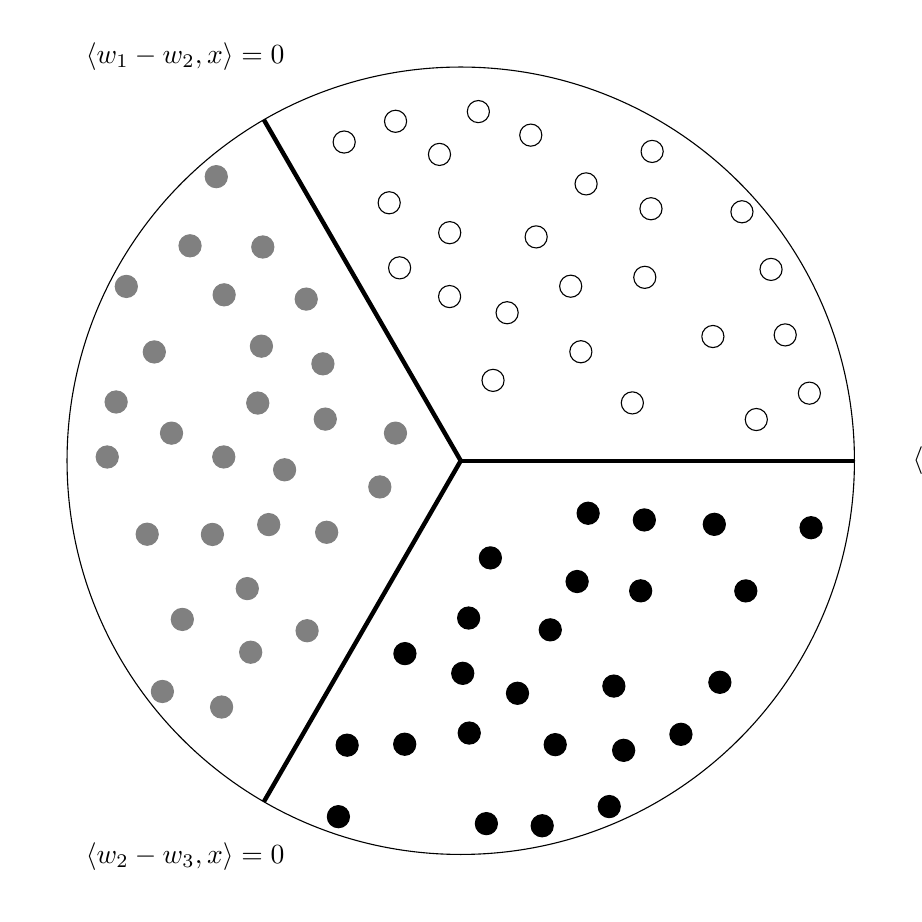
\begin{tikzpicture}

  \useasboundingbox (-5.5,-5.5) rectangle (5.5,5.5);
  % \draw[help lines] (-5.5,-5.5) rectangle (5.5,5.5);

  % Grid and coordinate axes
  %% \draw[help lines] (-5.2,-5.2) grid (5.2,5.2);
  %% \draw[thick, ->, >=latex] (-5.2,0) -- (5.2,0);
  %% \draw[thick, ->,  >=latex] (0,-5.2) -- (0,5.2);

  % Notable points
  \coordinate (Origin) at (0,0);

  \coordinate [label={[xshift=-10mm, yshift=5mm]$\ip{w_1 - w_2}{x} = 0$}] (A) at (120:5);
  \coordinate [label={[xshift=-10mm, yshift=-10mm]$\ip{w_2 - w_3}{x} = 0$}] (B) at (240:5);
  \coordinate [label={[xshift=+20mm, yshift=-3mm]$\ip{w_3 - w_1}{x} = 0$}] (C) at (360:5);

  % Circle which contains all the examples.
  \draw (Origin) circle (5);

  \draw[ultra thick] (Origin) -- (A);
  \draw[ultra thick] (Origin) -- (B);
  \draw[ultra thick] (Origin) -- (C);

  % Class 0 points. Angles between 0.0 and 120.0
  \draw[color=black, fill=none]
                    (7.94:3.79) circle (4pt)
                    (10.97:4.51) circle (4pt)
                    (18.63:2.30) circle (4pt)
                    (21.20:4.42) circle (4pt)
                    (26.23:3.57) circle (4pt)
                    (31.66:4.63) circle (4pt)
                    (41.52:4.77) circle (4pt)
                    (42.22:2.06) circle (4pt)
                    (44.90:3.30) circle (4pt)
                    (52.95:4.01) circle (4pt)
                    (57.79:2.62) circle (4pt)
                    (58.25:4.62) circle (4pt)
                    (65.64:3.86) circle (4pt)
                    (68.11:1.10) circle (4pt)
                    (71.38:3.00) circle (4pt)
                    (72.60:1.97) circle (4pt)
                    (77.86:4.23) circle (4pt)
                    (87.11:4.44) circle (4pt)
                    (92.77:2.90) circle (4pt)
                    (93.88:2.09) circle (4pt)
                    (93.97:3.90) circle (4pt)
                    (100.87:4.39) circle (4pt)
                    (105.50:3.40) circle (4pt)
                    (107.58:2.57) circle (4pt)
                    (110.09:4.31) circle (4pt)
                    ;

  % Class 1 points. Angles between 120.0 and 240.0
  \draw[color=gray, fill=gray]
                    (130.71:4.76) circle (4pt)
                    (132.80:3.70) circle (4pt)
                    (133.71:2.84) circle (4pt)
                    (141.55:4.39) circle (4pt)
                    (144.89:2.14) circle (4pt)
                    (144.96:3.67) circle (4pt)
                    (150.11:2.92) circle (4pt)
                    (152.47:4.79) circle (4pt)
                    (157.09:0.90) circle (4pt)
                    (160.45:4.13) circle (4pt)
                    (162.92:1.80) circle (4pt)
                    (164.13:2.68) circle (4pt)
                    (170.32:4.44) circle (4pt)
                    (174.55:3.69) circle (4pt)
                    (179.08:3.01) circle (4pt)
                    (179.39:4.49) circle (4pt)
                    (182.94:2.24) circle (4pt)
                    (193.19:4.09) circle (4pt)
                    (196.53:3.29) circle (4pt)
                    (197.93:1.08) circle (4pt)
                    (198.39:2.57) circle (4pt)
                    (208.08:1.93) circle (4pt)
                    (209.68:4.07) circle (4pt)
                    (210.92:3.16) circle (4pt)
                    (217.72:4.79) circle (4pt)
                    (222.35:3.61) circle (4pt)
                    (225.84:4.36) circle (4pt)
                    (227.89:2.91) circle (4pt)
                    ;

% Class 2 points. Angles between 240.0 and 360.0
  \draw[color=black, fill=black]
                    (248.23:3.89) circle (4pt)
                    (251.03:4.78) circle (4pt)
                    (253.86:2.55) circle (4pt)
                    (258.82:3.67) circle (4pt)
                    (270.54:2.70) circle (4pt)
                    (271.79:3.46) circle (4pt)
                    (272.88:2.00) circle (4pt)
                    (274.04:4.62) circle (4pt)
                    (282.58:4.75) circle (4pt)
                    (283.72:3.04) circle (4pt)
                    (286.97:1.29) circle (4pt)
                    (288.41:3.80) circle (4pt)
                    (293.24:4.78) circle (4pt)
                    (297.90:2.43) circle (4pt)
                    (299.36:4.22) circle (4pt)
                    (304.20:3.46) circle (4pt)
                    (308.83:4.46) circle (4pt)
                    (313.94:2.13) circle (4pt)
                    (319.47:4.33) circle (4pt)
                    (324.13:2.82) circle (4pt)
                    (335.46:3.98) circle (4pt)
                    (337.60:1.75) circle (4pt)
                    (342.13:2.45) circle (4pt)
                    (345.92:3.32) circle (4pt)
                    (349.18:4.53) circle (4pt)
                    ;

\end{tikzpicture}

\end{center}
\caption{The figure shows labeled examples in $\R^2$. The examples belong to
$K=3$ classes colored white, gray and black respectively. Each class lies in a
$120^\circ$ wedge. While the examples are linearly separable with a positive
margin $\gamma$, they are \emph{not} strongly linearly separable for any
positive margin $\gamma$.
}
\label{figure:linearly-separable-examples-with-margin}
\end{figure}


\section{Algorithm for strongly linearly separable data}
\label{section:algorithm-for-strongly-linearly-separable-data}

\begin{algorithm}[h]
\caption{\textsc{Bandit Algorithm for Strongly Linearly Separable Examples}
\label{algorithm:algorithm-for-strongly-linearly-separable-examples}}
\begin{algorithmic}[1]
{
\REQUIRE{Number of classes $K$. Number of rounds $T$. Inner product space $(V,\ip{\cdot}{\cdot})$.}
\STATE{Initialize $w_1^{(1)} = w_2^{(1)} = \dots = w_K^{(1)} = 0$}
\FOR{$t=1,2,\dots,T$}
\STATE{Observe feature vector $x_t \in V$}
\STATE{Compute $S_t = \left\{ i ~:~ 1 \le i \le K, \ \ip{w_i^{(t)}}{x_t} \ge 0 \right\}$}
\IF{$S_t = \emptyset$}
\STATE{Predict $\widehat y_t \sim \text{Uniform}(\{1,2,\dots,K\})$}
\ELSE
\STATE{Predict $\widehat y_t \sim \text{Uniform}(S_t)$}
\ENDIF
\STATE{Observe feedback $z_t \in \{0,1\}$ where $z_t = \indicator{\widehat y_t \neq y_t}$}
\IF{$S_t = \emptyset$}
\IF{$z_t = 1$}
\STATE{Set $w_i^{(t+1)} = w_i^{(t)}$ for all $i \in \{1,2,\dots,K\}$}
\ELSE
\STATE{Set $w_i^{(t+1)} = w_i^{(t)}$ for all $i \in \{1,2,\dots,K\} \setminus \{\widehat y_t\}$}
\STATE{Update $w_{\widehat y_t}^{(t+1)} = w_{\widehat y_t}^{(t)} + x_t$}
\ENDIF
\ELSE
\IF{$z_t = 1$}
\STATE{Set $w_i^{(t+1)} = w_i^{(t)}$ for all $i \in \{1,2,\dots,K\} \setminus \{\widehat y_t\}$}
\STATE{Update $w_{\widehat y_t}^{(t+1)} = w_{\widehat y_t}^{(t)} - x_t$}
\ELSE
\STATE{Set $w_i^{(t+1)} = w_i^{(t)}$ for all $i \in \{1,2,\dots,K\}$}
\ENDIF
\ENDIF
\ENDFOR
}
\end{algorithmic}
\end{algorithm}

\begin{theorem}
Let $(V, \ip{\cdot}{\cdot})$ be any inner product space, let $K$ be a positive
integer, $\gamma$ a positive real number, $R$ be a non-negative real number If
$(x_1, y_1), (x_2, y_2), \dots, (x_T, y_T)$ is a sequence of labeled examples in
$V \times \{1,2,\dots,K\}$ such that the examples are strongly separable with
margin $\gamma$ and $\norm{x_1}, \norm{x_2}, \dots, \norm{x_T} \le R$ then the
expected number of mistakes
Algorithm~\ref{algorithm:algorithm-for-strongly-linearly-separable-examples}
makes is at most $K(K-1) \lfloor (R/\gamma)^2 \rfloor$ mistakes.
\end{theorem}

\begin{proof}
Let $M = \sum_{t=1}^T z_t$ be the number of mistakes the algorithm makes. Let $A
= \sum_{t ~:~ S_t \neq \emptyset} z_t$ be the number of mistakes in the rounds
when $S_t \neq \emptyset$ and let $B = \sum_{t ~:~ S_t = \emptyset} z_t$ be the
number of mistakes in the rounds when $S_t = \emptyset$. Obviously, $M = A + B$.
We upper bound $A$ and $B$ separately.

Let $C$ be the number of times line 16 gets executed. Let $U$ be the number of
times line 16 or line 21 get executed. In other words, $U$ the number of times
the weight vectors are updated. Clearly, $U = A + C$. We know that $U \le
\frac{K} \lfloor (R/\gamma)^2 \rfloor$.

The key observation is that $\Exp[B] = (K-1) \Exp[C]$ since there the $1/K$
probability that the algorithm guesses the correct label correctly if $S_t =
\emptyset$. Putting all the information together, we get that
\begin{align*}
\Exp[M]
& = \Exp[A] + \Exp[B] \\
& = \Exp[A] + (K-1) \Exp[C]  \\
& \le (K-1) \Exp[A + C] \\
& = (K-1) \Exp[U]  \\
& \le K(K-1) \lfloor (R/\gamma)^2 \rfloor \; .
\end{align*}
\end{proof}


\section{Converting linear separability to strong linear separability}

TODO


\section{Nearest neighbor algorithm}

TODO


\section{NP-hardness of the weak labeling problem}

TODO


\section{Mistake lower bound for ignorant algorithms}

TODO

\bibliographystyle{plainnat}
\bibliography{biblio}

\appendix

\section{Multiclass Perceptron}
\label{section:multiclass-perceptron-proofs}

\textsc{Multiclass Perceptron} is an algorithm for \textsc{Online Multiclass
Classification}. Both the protocol for the problem and the algorithm are stated
below. The algorithm assumes that the feature vectors come from an inner product
space $(V, \ip{\cdot}{\cdot})$.

Two results are folklore. The first result is
\autoref{theorem:mutliclass-perceptron-mistake-upper-bound} which states that if
examples are linearly separable with margin $\gamma$ and examples have norm
at most $R$ then the algorithm makes at most $\lfloor 2 (R/\gamma)^2 \rfloor$
mistakes. The second result is
\autoref{theorem:online-multiclass-classification-mistake-lower-bound} which
states that under the same assumptions as in
\autoref{theorem:online-multiclass-classification-mistake-lower-bound}
\emph{any} deterministic algorithm for \textsc{Online Multiclass Classification}
must make at least $\lfloor (R/\gamma)^2 \rfloor$ mistakes in the worst case.

\begin{algorithm}[h]
\caption{\textsc{Online Multiclass Classification}
\label{algorithm:mutliclass-classification}}
\begin{algorithmic}[1]
{
\REQUIRE{Number of classes $K$. Number of rounds $T$.}
\FOR{$t=1,2,\dots,T$}
\STATE{Observe feature vector $x_t$}
\STATE{Predict $\widehat y_t \in \{1,2,\dots,K\}$}
\STATE{Observe $y_t \in \{1,2,\dots,K\}$}
\ENDFOR
}
\end{algorithmic}
\end{algorithm}

\begin{algorithm}[h]
\caption{\textsc{Multiclass Perceptron}
\label{algorithm:mutliclass-perceptron}}
\begin{algorithmic}[1]
{
\REQUIRE{Number of classes $K$. Number of rounds $T$. Inner product space $(V,\ip{\cdot}{\cdot})$.}
\STATE{Initialize $w_1^{(1)} = w_2^{(1)} = \dots = w_K^{(1)} = 0$}
\FOR{$t=1,2,\dots,T$}
\STATE{Observe feature vector $x_t \in V$}
\STATE{Predict $\widehat y_t = \argmax_{i \in \{1,2,\dots,K\}} \ip{w_t^{(i)}}{x_t}$}
\STATE{Observe $y_t \in \{1,2,\dots,K\}$}
\IF{$\widehat y_t \neq y_t$}
\STATE{Set $w_i^{(t+1)} = w_i^{(t)}$ for all $i \in \{1,2,\dots,K\} \setminus \{y_t, \widehat y_t\}$}
\STATE{Update $w_{y_t}^{(t+1)} = w_{y_t}^{(t)} + x_t$}
\STATE{Update $w_{\widehat y_t}^{(t+1)} = w_{\widehat y_t}^{(t)} - x_t$}
\ELSE
\STATE{Set $w_i^{(t+1)} = w_i^{(t)}$ for all $i \in \{1,2,\dots,K\}$}
\ENDIF
\ENDFOR
}
\end{algorithmic}
\end{algorithm}

\begin{theorem}[Mistake upper bound]
\label{theorem:mutliclass-perceptron-mistake-upper-bound}
Let $(V, \ip{\cdot}{\cdot})$ be an inner product space, let $K$ be a positive
integer, let $\gamma$ be a positive real number and let $R$ be a non-negative real
number. If $(x_1, y_1), (x_2, y_2), \dots, (x_T, y_T)$ is a sequence of labeled
examples in $V \times \{1,2,\dots,K\}$ that are linearly separable with margin
$\gamma$ and $\norm{x_1}, \norm{x_2}, \dots, \norm{x_T} \le R$
then \textsc{Multiclass Perceptron} algorithm makes at most $\lfloor
2(R/\gamma)^2 \rfloor$ mistakes.
\end{theorem}

\begin{proof}
Let $M = \sum_{t=1}^T \indicator{\widehat y_t \neq y_t}$ be the number of
mistakes the algorithm makes. Since the $K$-tuple $(w_1^{(t)}, w_2^{(t)}, \dots,
w_K^{(t)})$ changes only if a mistake is made, we can upper bound $\sum_{i=1}^K
\norm{w_i^{(t)}}^2$ in terms of number of mistakes.
If a mistake happens in round $t$,
\begin{align*}
\sum_{i=1}^K \norm{w_i^{(t+1)}}^2
& = \left(\sum_{i \in \{1,2,\dots,K\} \setminus \{y_t, \widehat y_t\} } \norm{w_i^{(t)}}^2 \right) + \norm{w_{y_t}^{(t)} + x_t}^2 + \norm{w_{\widehat y_t}^{(t)} - x_t}^2 \\
& = \left(\sum_{i \in \{1,2,\dots,K\} \setminus \{y_t, \widehat y_t\} } \norm{w_i^{(t)}}^2 \right) + \norm{w_{y_t}^{(t)}}^2 + \norm{w_{\widehat y_t}^{(t)}}^2 + 2 \norm{x_t}^2 + 2 \ip{w_{y_t}^{(t)} - w_{\widehat y_t}^{(t)}}{x_t} \\
& = \left(\sum_{i=1}^K \norm{w_i^{(t)}}^2 \right) + 2 \norm{x_t}^2 + 2 \ip{w_{y_t}^{(t)} - w_{\widehat y_t}^{(t)}}{x_t} \\
& \le \left(\sum_{i=1}^K \norm{w_i^{(t)}}^2 \right) + 2 \norm{x_t}^2 \\
& \le \left(\sum_{i=1}^K \norm{w_i^{(t)}}^2 \right) + 2 R^2 \; .
\end{align*}
So each time a mistake happens, $\sum_{i=1}^K \norm{w_i^{(t)}}^2$ increases by at most $2R^2$. Thus,
$$
\sum_{i=1}^K \norm{w_i^{(T+1)}}^2 \le 2R^2 M \; .
$$
Let $w_1^*, w_2^*, \dots, w_K^* \in V$ be vectors satisfying the
\eqref{equation:linear-separability-1} and
\eqref{equation:linear-separability-2}. We lower bound $\sum_{i=1}^K \ip{w_i^*}{w_i^{(t)}}$. This quantity changes
only when a mistakes happens. If mistake happens in round $t$, we have
\begin{align*}
\sum_{i=1}^K \ip{w_i^*}{w_i^{(t+1)}}
& = \left( \sum_{i \in \{1,2,\dots,K\} \setminus {y_t, \widehat y_t}} \ip{w_i^*}{w_i^{(t)}} \right) + \ip{w_{y_t}^*}{w_{y_t}^{(t)} + x_t} + \ip{w_{\widehat y_t}^*}{w_{\widehat y_t}^{(t)} - x_t} \\
& = \left( \sum_{i=1}^K \ip{w_i^*}{w_i^{(t)}} \right) + \ip{w_{y_t}^* - w_{\widehat y_t}^*}{x_t} \\
& \ge  \left( \sum_{i=1}^K \ip{w_i^*}{w_i^{(t)}} \right) + \gamma \; .
\end{align*}
Thus, after $M$ mistakes,
$$
\sum_{i=1}^K \ip{w_i^*}{w_i^{(T+1)}} \ge \gamma M \; .
$$
We upper bound the left hand side by using Cauchy-Schwartz inequality twice and
the condition \eqref{equation:linear-separability-1} on $w_1^*, w_2^*, \dots,
w_K^*$. We have
$$
\sum_{i=1}^K \ip{w_i^*}{w_i^{(T+1)}}
\le \sum_{i=1}^K \norm{w_i^*} \cdot \norm{w_i^{(T+1)}}
\le \sqrt{\sum_{i=1}^K \norm{w_i^*}^2} \sqrt{\sum_{i=1}^K \norm{w_i^{(T+1)}}^2}
\le \sqrt{\sum_{i=1}^K \norm{w_i^{(T+1)}}^2} \; .
$$
Combining all inequalities, we get
$$
(\gamma M)^2 \le \sum_{i=1}^K \norm{w_i^{(T+1)}}^2 \le 2R^2 M \; .
$$
We conclude that $M \le 2(R/\gamma)^2$. Since $M$ is an integer, $M \le \lfloor 2(R/\gamma)^2 \rfloor$.
\end{proof}


\begin{theorem}[Mistake lower bound]
\label{theorem:online-multiclass-classification-mistake-lower-bound}
Let $K$ be a positive integer, let $\gamma$ be a positive real number and let
$R$ be a non-negative real number. For any deterministic algorithm for the
\textsc{Full-Information Multiclass Classification} problem there exists an
inner product space $(V, \ip{\cdot}{\cdot})$, a non-negative integer $T$ and a
sequence of labeled examples $(x_1, y_1), (x_2, y_2), \dots, (x_T, y_T)$
examples in $V \times \{1,2,\dots,K\}$ that are linearly separable with margin
$\gamma$, the norms satisfy $\norm{x_1}, \norm{x_2}, \dots, \norm{x_T} \le R$
and the algorithm makes at least $\lfloor (R/\gamma)^2 \rfloor$ mistakes.
\end{theorem}

\begin{proof}
Let $T = \lfloor (R/\gamma)^2 \rfloor$ and let $x_1, x_2, \dots, x_T$ be the
orthogonal vectors such that $\norm{x_t} = R$ for all $t=1,2,\dots,T$. For
example, we can take $V = \R^T$ and $x_t = R e_t$ where $e_t$ is $t$-th element
of the standard orthonormal basis of $\R^T$.

Since the algorithm is deterministic, we can construct the sequence of labels
$y_1, y_2, \dots, y_T$ adaptively based on the predictions $\widehat y_1,
\widehat y_2, \dots, \widehat y_T$ of the algorithm. We define $y_t$ to be any
element of $\{1,2,\dots,K\}$ not equal to $\widehat y_t$. This way the algorithm
makes a mistake in every round $t=1,2,\dots,T$.

It remains to show that the examples we have constructed are linearly separable
with margin $\gamma$. To prove that we demostrate vectors $w_1, w_2, \dots, w_K$
satisfying conditions \eqref{equation:linear-separability-1} and
\eqref{equation:linear-separability-2}. We define
$$
w_i = \frac{1}{R\sqrt{T}} \sum_{\substack{t : 1 \le t \le T \\ y_t = i}} x_t \qquad \qquad \text{for $i=1,2,\dots,K$.}
$$
Let $a_i = |\{ t ~:~ 1 \le t \le T, \ y_t = i \}|$ be the number of occurences of label $i$.
It is easy to see that
$$
\norm{w_i}^2 = \frac{1}{R^2 T} \sum_{\substack{t : 1 \le t \le T \\ y_t = i}} \norm{x_t}^2 = \frac{a_i}{T} \qquad \qquad \text{for $i=1,2,\dots,K$.}
$$
Since $\sum_{i=1}^K a_i = T$, the condition
\eqref{equation:linear-separability-1} holds. To verify condition
\eqref{equation:linear-separability-2} consider any labeled example $(x_t,
y_t)$. Then, by definition of $w_{y_t}$ we have
$$
\ip{w_{y_t}}{x_t}
= \frac{1}{R\sqrt{T}} \sum_{\substack{s : 1 \le s \le T \\ y_s = y_t}} \ip{x_s}{x_t}
= \frac{1}{R\sqrt{T}} \norm{x_t}^2
= \frac{R}{\sqrt{T}}
\ge \frac{R}{R/\gamma}
= \gamma \; .
$$
and for any $i \in \{1,2,\dots,K\} \setminus \{y_t\}$ we have
$\ip{w_i}{x_t} = 0$. Therefore, condition \eqref{equation:linear-separability-2} holds.
\end{proof}

\end{document}
